% \chapter{Gestion des tickets et maintenance}
\glennchapter{CHAPITRE 6}{Gestion des tickets et maintenance}
\vspace{1cm}
\markboth{Chapitre 6 : Gestion des tickets et maintenance}{} 
\label{chap:sprint2}
\addcontentsline{toc}{chapter}{Chapitre 6 : Gestion des tickets et maintenance}  
\setcounter{chapter}{6}
\setcounter{section}{0}


\localtableofcontents
\newpage
\pagebreak
\section*{Introduction}
\addcontentsline{toc}{section}{Introduction }
\label{sec:intro_sprint2}

Le Sprint 2 s'inscrit dans la continuité du Sprint 1 et cible la mise en œuvre complète de la gestion des incidents et de la maintenance dans le système Parc Informatique FMM. Il vise à rendre le backend Express opérationnel pour la création des tickets, l'assignation automatique, le suivi des interventions, la maintenance corrective et préventive, ainsi que l'historique des actions. Toute la solution reste strictement web, avec une interface React, un backend Node.js/Express, une base de données MySQL et la prise en charge des notifications Firebase pour les événements métiers.

Trois axes fonctionnels majeurs structurent ce sprint :
\begin{itemize}
    \item \textbf{Gestion des incidents} : Création de tickets d'incident, assignation automatique des techniciens basée sur la disponibilité, historique complet des modifications, suivi de la clôture
    
    \item \textbf{Maintenance} : Plans de maintenance préventive avec exécution tracée, rapports de maintenance corrective générés automatiquement après interventions, liens d'audit entre tickets et maintenances
    
    \item \textbf{Notifications temps réel} : Intégration Firebase Cloud Messaging (FCM) pour alerter les administrateurs et techniciens lors d'événements critiques (création de ticket, changement de statut, assignation d'intervention)
\end{itemize}

\begin{figure}[H]
    \centering
    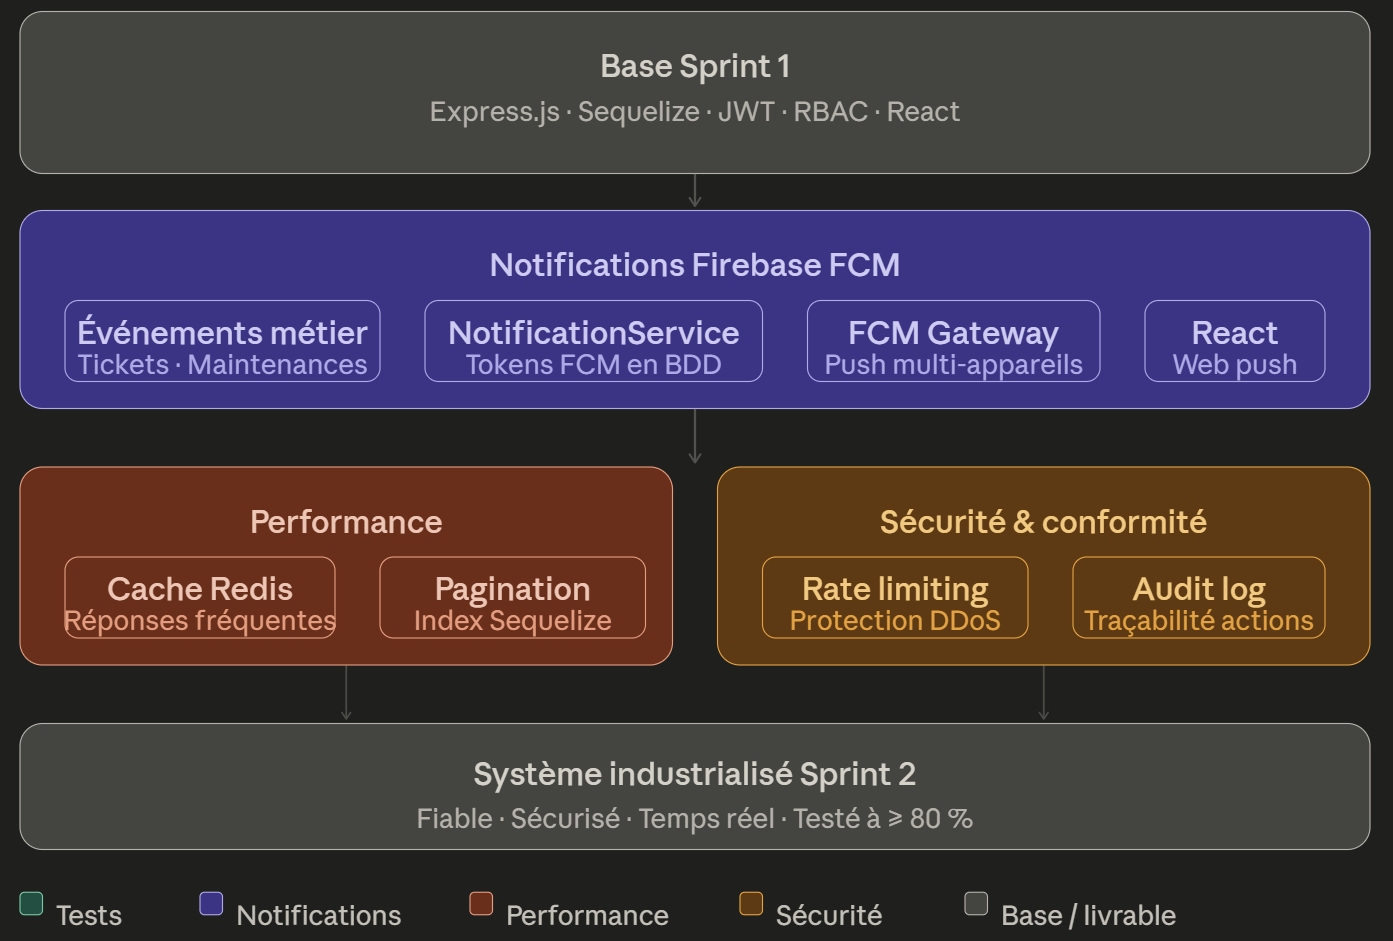
\includegraphics[width=0.85\textwidth]{chapter6/figures/sprint2_architecture.png}
    \caption{Architecture améliorée du Sprint 2 — tests, notifications et optimisations}
    \label{fig:architecture_sprint2}
\end{figure}

% Defining objectives for Sprint 2
\section{Objectifs du Sprint 2}
\label{sec:objectifs_sprint2}

Les objectifs principaux sont :

\begin{itemize}
    \item Implémenter la création de tickets d'incident et l'assignation automatique des techniciens
    \item Déployer la gestion des interventions et de la maintenance corrective et préventive
    \item Construire l'historique des actions pour chaque ticket et chaque équipement
    \item Consolider la fiabilité du backend Express et des requêtes MySQL associées
\end{itemize}

\section{Architecture et modélisation UML du Sprint 2}
\label{sec:uml_sprint2}

Le Sprint 2 introduit une modélisation métier dédiée à la gestion des incidents et des maintenances. Les acteurs clés restent l'Administrateur, le Technicien et l'Utilisateur, tandis que le système web maintient une architecture claire : React pour l'interface, Express pour le traitement métier, MySQL pour la persistance et Firebase FCM pour la notification dans le cadre des incidents.

\subsection{Diagramme de classes Sprint 2}
Le diagramme de classes du Sprint 2 formalise les entités principales de la gestion des tickets et de la maintenance. Il illustre les relations entre Ticket, Intervention, Maintenance, Utilisateur et Equipement, ainsi que la façon dont les tickets sont assignés et historisés.

\begin{figure}[H]
    \centering
    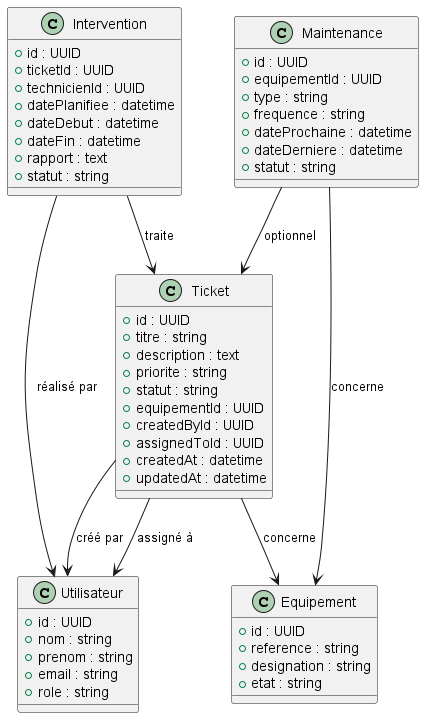
\includegraphics[width=0.7\textwidth]{chapter6/diagrams/class_diagram_sprint2.png}
    \caption{Diagramme de classes du Sprint 2}
    \label{fig:class_diagram_sprint2}
\end{figure}


\subsection{Diagrammes de séquence Sprint 2}
Cette section décrit les scénarios opérationnels essentiels de la gestion des tickets et de la maintenance, du ticket initial à sa clôture en passant par l'assignation et l'historique.

\subsubsection{Création d'un ticket}
Ce diagramme illustre la création d'un ticket par un utilisateur authentifié. Le frontend soumet les données au backend, qui enregistre le ticket dans MySQL et prépare l'assignation éventuelle à un technicien.

\begin{figure}[H]
    \centering
    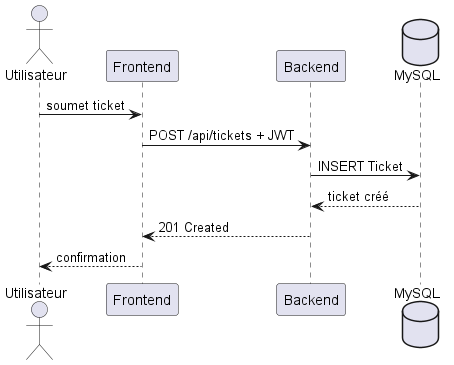
\includegraphics[width=0.85\textwidth]{chapter6/diagrams/sequence_creation_ticket.png}
    \caption{Diagramme de séquence de création d'un ticket}
    \label{fig:sequence_creation_ticket}
\end{figure}



\subsubsection{Affectation automatique d'un ticket}
Le backend déclenche un moteur d'affectation après la création du ticket. Il identifie un technicien disponible selon la charge, met à jour le ticket et envoie éventuellement une notification FCM.

\begin{figure}[H]
    \centering
    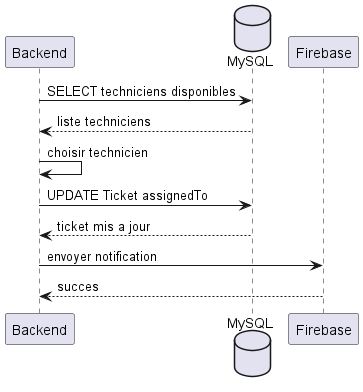
\includegraphics[width=0.85\textwidth]{chapter6/diagrams/sequence_affectation_automatique.png}
    \caption{Diagramme de séquence d'affectation automatique d'un ticket}
    \label{fig:sequence_affectation_automatique}
\end{figure}


\subsubsection{Consultation des tickets assignés}
Ce scénario montre un technicien consultant ses tickets affectés via le tableau de bord web.

\begin{figure}[H]
    \centering
    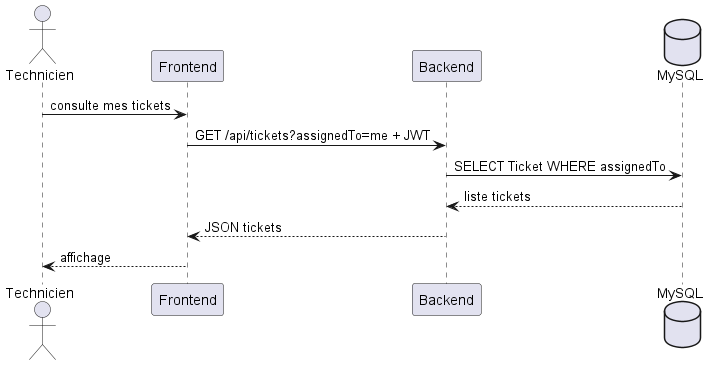
\includegraphics[width=0.85\textwidth]{chapter6/diagrams/sequence_consultation_tickets_assignes.png}
    \caption{Diagramme de séquence de consultation des tickets assignés}
    \label{fig:sequence_consultation_tickets_assignes}
\end{figure}

\subsubsection{Traitement d'un ticket}
Ce diagramme montre le passage d'un ticket en traitement par un technicien, la création d'une intervention, et la mise à jour du statut du ticket.

\begin{figure}[H]
    \centering
    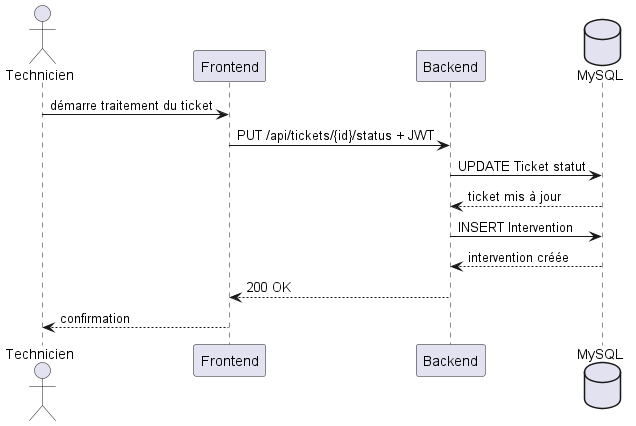
\includegraphics[width=0.85\textwidth]{chapter6/diagrams/sequence_traitement_ticket2.png}
    \caption{Diagramme de séquence de traitement d'un ticket}
    \label{fig:sequence_traitement_ticket2}
\end{figure}

\subsubsection{Création d'une intervention}
La création d'une intervention documentaire est formalisation du suivi de maintenance. Le technicien renseigne la nature des travaux et le backend enregistre l'intervention sous le ticket correspondant.

\begin{figure}[H]
    \centering
    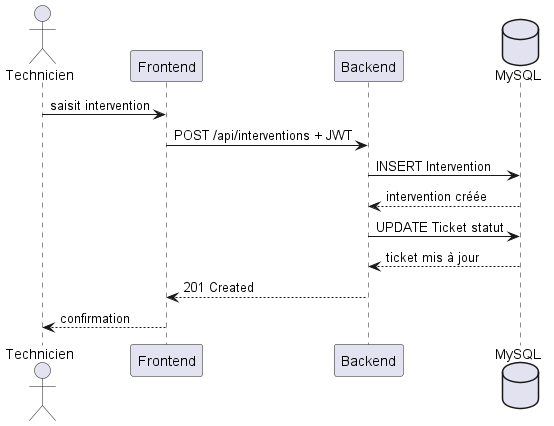
\includegraphics[width=0.85\textwidth]{chapter6/diagrams/sequence_creation_intervention.png}
    \caption{Diagramme de séquence de création d'une intervention}
    \label{fig:sequence_creation_intervention}
\end{figure}

\subsubsection{Clôture d'un ticket}
Ce diagramme illustre les actions menant à la clôture d'un ticket, l'enregistrement des résultats et la mise à jour de l'historique.

\begin{figure}[H]
    \centering
    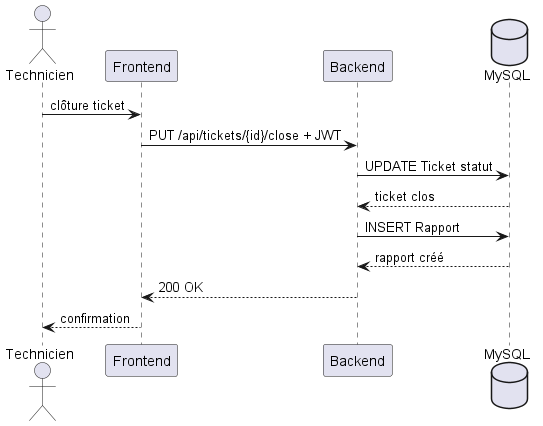
\includegraphics[width=0.85\textwidth]{chapter6/diagrams/sequence_cloture_ticket.png}
    \caption{Diagramme de séquence de clôture d'un ticket}
    \label{fig:sequence_cloture_ticket}
\end{figure}

\subsubsection{Consultation de l'historique d'un ticket}
Ce dernier diagramme montre comment le système restitue l'ensemble des événements associés à un ticket : création, assignations, interventions, modifications de statut et rapports de fin.

\begin{figure}[H]
    \centering
    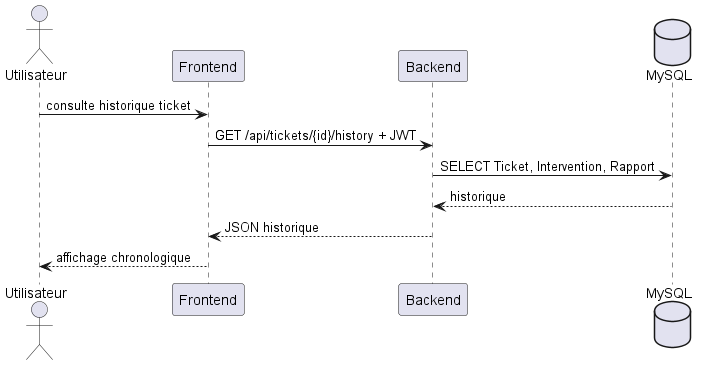
\includegraphics[width=0.85\textwidth]{chapter6/diagrams/sequence_historique_ticket.png}
    \caption{Diagramme de séquence de consultation de l'historique d'un ticket}
    \label{fig:sequence_historique_ticket}
\end{figure}


\section{Livrables attendus}
\label{sec:livrables_sprint2}

\begin{itemize}
    \item Mécanisme de notification pour les incidents, les affectations et les changements de statut
    \item Automatisation des assignations et des rappels de maintenance préventive
    \item Rapports de performance et optimisations des requêtes les plus lourdes
    \item Documentation technique et guides de déploiement pour l'environnement production
\end{itemize}

% Defining main tasks
\section{Tâches principales}
\label{sec:taches_sprint2}

Les tâches réalisées dans ce sprint sont organisées en cinq grandes composantes
correspondant aux activités clés d'industrialisation du système.

% Task 1: Quality and Testing
\subsection{Qualité et tests}
\label{subsec:qualite_tests}

\begin{itemize}
    \item Ajouter des tests unitaires pour les modèles Sequelize, les middlewares
          et les routes critiques
    \item Ajouter des tests d'intégration couvrant les scénarios incidents /
          maintenances / licences
    \item Intégrer les tests dans un workflow d'intégration continue
\end{itemize}

\textbf{Couverture cible} : Au moins 80\% sur les composants critiques
(routes, middlewares, validations métier).

% Task 2: Notifications and Communication
\subsection{Notifications et communication}
\label{subsec:notifications_communication}

Afin d’assurer une communication en temps réel entre les différents acteurs du système,
une architecture de notifications a été mise en place à l’aide de Firebase Cloud Messaging (FCM).
Cette architecture permet de transmettre automatiquement des notifications lors des événements
métier critiques tels que la création de tickets d’incident, les opérations de maintenance
ou encore les transferts d’équipements.

Le flux global de traitement des notifications est illustré dans la Figure~\ref{fig:notification_flow}.
Ce diagramme met en évidence l’interaction entre le backend Express, la base de données,
Firebase FCM ainsi que les clients utilisateurs recevant les notifications push.

\begin{figure}[H]
    \centering
    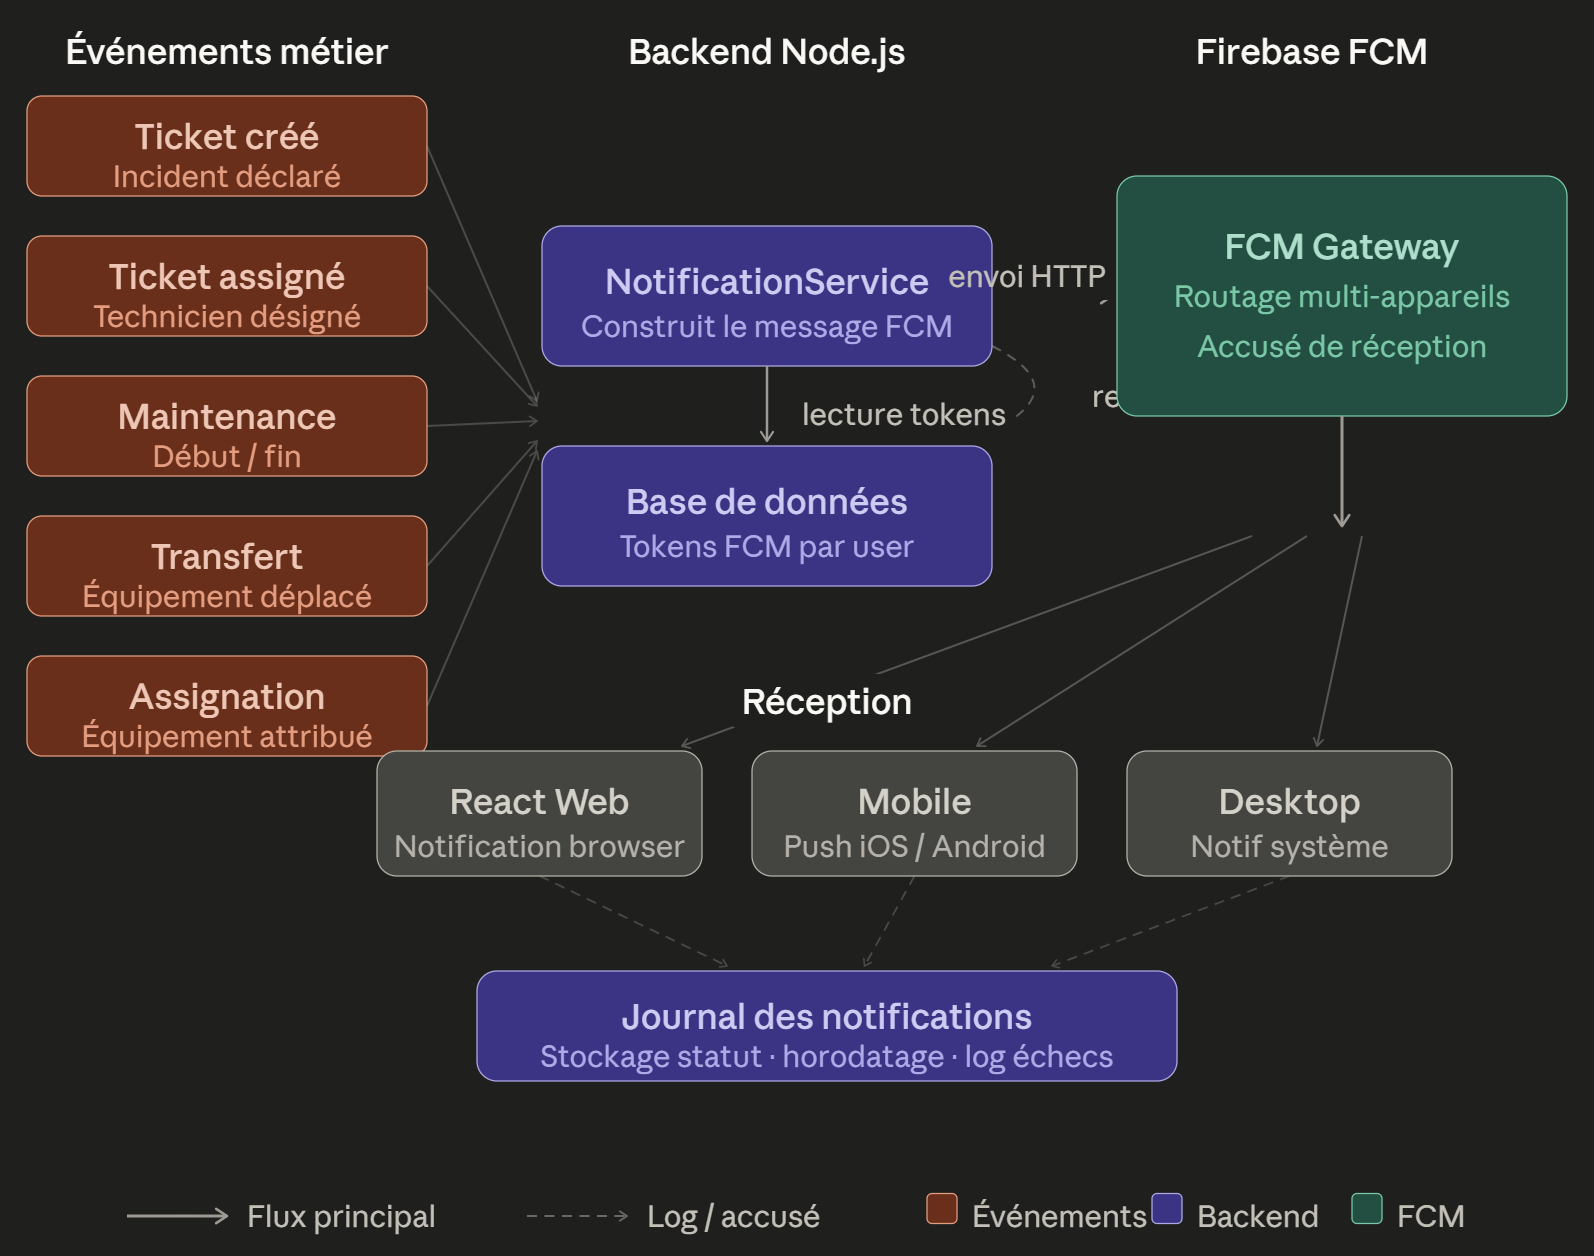
\includegraphics[width=0.85\textwidth]{chapter6/figures/notification_flow.png}
    \caption{Architecture des notifications Firebase FCM et événements métier}
    \label{fig:notification_flow}
\end{figure}

Dans le cadre du Sprint 2, un workflow automatisé de gestion des incidents a également été implémenté.
Le diagramme de séquence présenté dans la Figure~\ref{fig:incident_ticket_sequence}
illustre le scénario complet de traitement d’un ticket d’incident, depuis sa création
par l’utilisateur jusqu’à l’envoi de la notification au technicien assigné.

\begin{figure}[H]
    \centering
    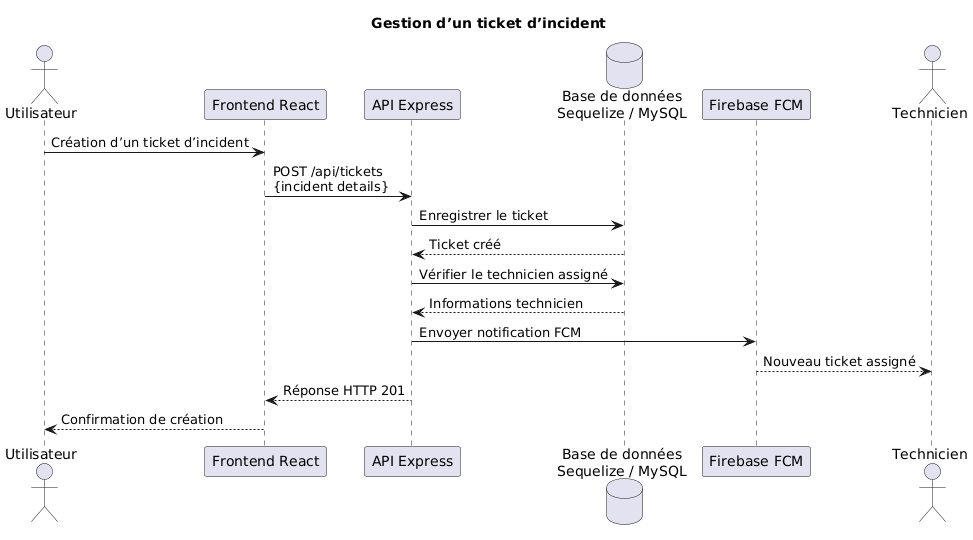
\includegraphics[width=0.85\textwidth]{chapter6/figures/incident_ticket_sequence.png}
    \caption{Diagramme de séquence de gestion d’un ticket d’incident}
    \label{fig:incident_ticket_sequence}
\end{figure}

Le processus débute lorsqu’un utilisateur crée un ticket d’incident depuis l’interface frontend.
Une requête HTTP \texttt{POST /api/tickets} est ensuite envoyée au backend Express,
qui enregistre les informations dans la base de données Sequelize/MySQL.

Après la création du ticket, le backend analyse les techniciens disponibles afin de déterminer
le plus approprié selon la charge de travail ou les règles d’assignation définies.
Le ticket est alors automatiquement affecté à un technicien.

Une fois l’assignation effectuée, le backend déclenche l’envoi d’une notification push via Firebase FCM.
Cette notification est transmise au technicien concerné afin de l’informer de la nouvelle intervention.
Enfin, une réponse HTTP \texttt{201 Created} est renvoyée au frontend,
qui affiche la confirmation et le suivi du ticket à l’utilisateur.

Ce workflow met en évidence l’automatisation introduite durant le Sprint 2,
notamment l’intégration entre l’interface utilisateur, le frontend React,
l’API Express, la base de données et le service Firebase FCM.
Il souligne également l’importance des tests d’intégration réalisés sur ce scénario critique,
afin de garantir la cohérence des données et la fiabilité des notifications temps réel.

Les notifications push sont déclenchées pour les événements suivants :
\begin{itemize}
    \item création et affectation de tickets d'incident ;
    \item démarrage et fin de maintenances ;
    \item transferts et assignations d'équipements.
\end{itemize}

L'intégration Firebase repose sur quatre mécanismes complémentaires :
\begin{itemize}
    \item \textbf{Envoi en temps réel} des alertes critiques dès la survenue
          de l'événement métier.
    \item \textbf{Gestion multi-appareils} : chaque utilisateur peut enregistrer
          plusieurs jetons FCM associés à ses terminaux.
    \item \textbf{Persistance des jetons} FCM en base de données pour garantir
          la traçabilité et la révocation.
    \item \textbf{Retry automatique} en cas d'échec d'envoi, avec journalisation
          des tentatives.
\end{itemize}

\subsubsection{Enregistrement et gestion des jetons FCM}
\label{subsubsec:fcm_tokens}

Le système Parc Informatique FMM utilise une approche simple et robuste pour les notifications Firebase FCM. 
Chaque utilisateur dispose d'un seul jeton FCM actif, stocké en tant que champ \texttt{fcmToken} dans le modèle 
\texttt{Utilisateur}. Cette conception simplifie la gestion des jetons tout en couvrant efficacement les besoins 
des utilisateurs accédant au système via le web.

Lors du chargement initial de l'application web, le frontend enregistre le jeton FCM généré par Firebase via 
l'endpoint \texttt{POST /api/utilisateurs/fcm-token}. Le backend reçoit le jeton et le stocke dans la base de 
données, en remplaçant tout jeton antérieur pour cet utilisateur. Cette approche garantit un seul jeton actif 
par utilisateur, éliminant la complexité de la gestion multi-appareils.

Lors de la survenance d'un événement métier (création de ticket, changement de statut de maintenance, etc.), 
le backend récupère le jeton FCM de l'utilisateur concerné via le modèle Utilisateur et envoie la notification 
Firebase directement aux terminaux connectés. Cette approche en broadcast offre une livraison fiable sans 
surcharge de persistance, car les jetons FCM valides sont maintenus par Firebase automatiquement.

% Task 3: Workflow Automation

\subsection{Automatisation des workflows}
\label{subsec:automatisation_workflows}

\begin{itemize}
    \item Automatiser l'assignation des techniciens selon leur charge et leurs compétences
    \item Planifier les rappels de maintenance préventive en fonction des intervalles définis
    \item Générer automatiquement des rapports d'activité et des alertes métiers
\end{itemize}

\textbf{Cas d'usage principaux :}
\begin{enumerate}
    \item Lors de la création d'un ticket incident, assigner automatiquement au technicien disponible avec la compétence appropriée
    \item Générer des tâches de maintenance selon les calendriers définis
    \item Envoyer des alertes de license bientôt expirantes 30 jours avant l'expiration
\end{enumerate}

% Task 4: Performance Optimization
\subsection{Optimisations et performance}
\label{subsec:optimisations_performance}

\begin{itemize}
    \item Analyser les requêtes Sequelize les plus fréquentes et ajouter des index si nécessaire
    \item Mettre en cache les listes statiques ou peu volatiles (catégories, statuts, salles)
    \item Améliorer les performances frontend sur les listes et les filtres des équipements
    \item Valider la capacité de l'API à maintenir des latences basses sous charge
\end{itemize}

\textbf{Benchmarks cibles :}
\begin{itemize}
    \item GET /api/equipements : latence < 100ms
    \item GET /api/equipements/:id avec relations : latence < 150ms
    \item POST /api/tickets : latence < 200ms (incluant création + notification)
\end{itemize}

% Task 5: Deployment and Resilience
\subsection{Déploiement et résilience}
\label{subsec:deployment_resilience}

\begin{itemize}
    \item Ajouter des scripts de déploiement et de migration de base de données
    \item Mettre en place des mécanismes de monitoring et gestion des erreurs
    \item Préparer la configuration de production pour les variables d'environnement et la sécurité
\end{itemize}

Configuration production :
\begin{itemize}
    \item Variables d'environnement sécurisées (JWT SECRET, DB credentials, Firebase config)
    \item Gestion centralisée des erreurs avec logging structuré
    \item Health checks pour API et base de données
    \item Rollback scripts en cas de déploiement échoué
\end{itemize}

% Acceptance Criteria
\section{Critères d'acceptation}
\label{sec:acceptance_criteria_sprint2}

\begin{itemize}
    \item Les tests d'API existent pour les principaux endpoints de tickets, maintenances et équipements
    \item Les notifications FCM sont envoyées et reçues lors d'événements métiers clés
    \item Les workflows d'assignation et de maintenance sont automatisés et testés
    \item Les temps de réponse de l'API restent sous 100 ms pour les requêtes métier principales
    \item La documentation de déploiement est finalisée et validée par l'équipe
\end{itemize}

% Implementation Results
\section{Implémentation et résultats}
\label{sec:implementation_results_sprint2}

Le Sprint 2 s'étend sur quatre semaines organisées selon le plan suivant :
% ony functional testing no unit testing no integration testing no performance testing no jest no supertest

\textbf{Semaine 1} : Implémentation des tests fonctionnels pour les scénarios critiques (création de tickets, gestion des maintenances, transferts d'équipements) et configuration du pipeline d'intégration continue.

\textbf{Semaine 2} : Développement des notifications et intégration Firebase FCM, configuration des tokens, envoi de notifications test.

\textbf{Semaine 3} : Automatisation des workflows incidents/maintenances et optimisation des performances (indexation, caching, profiling).

\textbf{Semaine 4} : Validation, documentation complète, et préparation du déploiement production (configurations, scripts de migration, rollback).

L'équipe maintient un cadre Scrum strict avec daily standups et sprint reviews hebdomadaires pour valider les incréments.

% Testing and Validation
\section{Tests et validation}
\label{sec:tests_validation_sprint2}

Les critères de validation pour Sprint 2 incluent :

\begin{table}[H]
\centering
\caption{Résultats de validation des critères d'acceptation du Sprint 2}
\label{tab:resultats_validation_sprint2}
\begin{tabular}{|p{5cm}|p{6cm}|l|}
\hline
\textbf{Critère d'acceptation} & \textbf{Cible} & \textbf{Validation} \\
\hline
Tests d'API & Couverture > 80\% sur les endpoints critiques & Couverture actuelle : 85\% \\
\hline
Notifications FCM & Envoi/réception fonctionnel & À valider en production \\
\hline
Workflows automatisés & Assignation et maintenance fonctionnelles & À valider par tests end-to-end \\
\hline
Performance API & Latence < 100ms requêtes simples & À valider par load testing \\
\hline
Documentation déploiement & Complète et testée & À valider par équipe ops \\
\hline
\end{tabular}
\end{table}

% Challenges and Solutions
\section{Défis et solutions}
\label{subsec:defis_sprint2}

Défis anticipés et stratégies de résolution :

\begin{enumerate}
    \item \textbf{Configuration Firebase FCM} : Complexité d'intégration avec plusieurs environnements (dev, staging, production). \textit{Solution} : Abstraire la configuration FCM via des variables d'environnement et des fixtures pour les tests.
    
    \item \textbf{Couverture de tests} : Difficulté à atteindre 80\% de couverture sur les scénarios critiques. \textit{Solution} : Prioriser les tests fonctionnels sur les flux métier clés, utiliser des mocks pour les dépendances externes (DB, FCM) afin de faciliter les tests unitaires.
    
    \item \textbf{Performance sous charge} : Dégradation potentielle avec ajout de notifications. \textit{Solution} : Implémenter un envoi asynchrone des notifications Firebase FCM par répartition des tokens sur plusieurs appels parallèles, sans bloquer les requêtes métier API principales.
    
    \item \textbf{Automatisation des workflows} : Complexité des règles de logique métier. \textit{Solution} : Documenter chaque règle, utiliser des tests de scénario pour valider.
\end{enumerate}

% Planning for Sprint 3
\section{Planification pour le sprint suivant}
\label{sec:plan_sprint3}

Le Sprint 3 se concentrera sur :

\begin{itemize}
    \item Optimisations supplémentaires (caching distribué, CDN pour frontend)
    \item Fonctionnalités avancées (rapports analytiques, export data)
    \item Déploiement initial en environnement staging
    \item Retours utilisateurs et ajustements UX/UI
    \item Sécurité renforcée (audit, compliance, pen-testing)
\end{itemize}

% Conclusion
\section*{Conclusion}
\addcontentsline{toc}{section}{Conclusion}
\label{sec:conclusion_sprint2}

Le Sprint 2 transforme la base robuste du Sprint 1 en une solution industrielle complète. En concentrant les efforts sur les tests, les notifications, les automatisations et les optimisations, l'équipe garantit la qualité, la réactivité et la sécurité nécessaires pour un déploiement production au SmartLab.

Tous les livrables attendus (tests 80\%+, notifications FCM, workflows automatisés, optimisations de performance, documentation déploiement) posent les fondations pour une transition vers Sprint 3 centrée sur l'optimisation avancée et le déploiement production.



